\documentclass[sigconf,natbib=true,anonymous=true,review=true]{acmart}

\usepackage{tikz}
\usetikzlibrary{
    calc,
    arrows.meta,
    shapes.misc,
    positioning
}

% CIKM 2026 short-paper track: 2-column ACM sigconf, 4 pages of main content
% including any appendix, plus unlimited pages for GenAI disclosure and references.
% For camera-ready, remove anonymous=true and review=true, then fill author blocks.

\settopmatter{printacmref=false}
\setcopyright{none}
\renewcommand\footnotetextcopyrightpermission[1]{}

\usepackage{amsmath,amssymb,mathtools}
\usepackage{booktabs}
\usepackage{enumitem}
\usepackage{xspace}

\newcommand{\PGF}{\mathrm{PGF}\xspace}
\newcommand{\E}{\mathbb{E}}
\newcommand{\N}{\mathbb{N}}
\newcommand{\R}{\mathbb{R}}
\newcommand{\C}{\mathbb{C}}
\newcommand{\jj}{\mathrm{i}}
\newcommand{\todo}[1]{\textcolor{red}{[TODO: #1]}}

\title{Scalable Poisson Mixture Learning from Probability-Generating Function Sketches}

\author{Anonymous Author(s)}
\affiliation{%
  \institution{Anonymous Institution}
  \city{Anonymous City}
  \country{Anonymous Country}}
\email{anonymous@example.com}

\begin{document}

\begin{abstract}
Mixtures of Poisson distributions are widely used to model heterogeneous count data, but classical likelihood-based inference can be costly on large datasets and sensitive to initialization. 
We study a compressed alternative based on empirical probability-generating-function sketches. 
The key observation is that, when the PGF of a finite mixed Poisson model is sampled along complex lines, the resulting measurements form multidimensional sums of exponentials. 
We exploit this structure with a joint ESPRIT recovery procedure: a global multi-snapshot subspace is estimated from several sampling directions, rotational invariance matrices are jointly diagonalized, and Poisson rates are recovered by a small wrapped least-squares problem, and mixture weights by constrained least squares.
Compared with marginal PGF--ESPRIT pipelines, the joint formulation avoids a combinatorial cross-coordinate alignment step and directly targets multidimensional components. 
Our experiments distinguish two questions: algorithmic comparisons under the same finite product-Poisson mixture model, and model-level comparisons involving alternative count-data models such as Poisson--Gamma variants. 
\todo{Replace this sentence by the final quantitative summary: runtime, PGF error, Hellinger/chi-square distances, and parameter recovery error.}
\end{abstract}

\begin{CCSXML}
<ccs2012>
<concept>
<concept_id>10010147.10010257.10010258.10010260</concept_id>
<concept_desc>Computing methodologies~Bayesian network models</concept_desc>
<concept_significance>300</concept_significance>
</concept>
<concept>
<concept_id>10002951.10003227.10003251</concept_id>
<concept_desc>Information systems~Data mining</concept_desc>
<concept_significance>500</concept_significance>
</concept>
<concept>
<concept_id>10002950.10003705.10003708</concept_id>
<concept_desc>Mathematics of computing~Probabilistic algorithms</concept_desc>
<concept_significance>300</concept_significance>
</concept>
</ccs2012>
\end{CCSXML}

\ccsdesc[500]{Information systems~Data mining}
\ccsdesc[300]{Mathematics of computing~Probabilistic algorithms}
\ccsdesc[300]{Computing methodologies~Mixture models}

\keywords{data sketching, Poisson mixtures, count data, probability generating functions, ESPRIT, joint diagonalization}

\maketitle

\section{Introduction}

Many datasets consist of nonnegative integer-valued observations: numbers of events, interactions, messages, visits, reads, or molecular counts. 
Finite mixtures of Poisson distributions provide a simple and interpretable model for such data. 
They describe heterogeneous populations through a finite number of latent components, each associated with a Poisson rate vector and a mixture weight. 
Estimating these parameters is a classical latent-variable inference problem, most commonly addressed through maximum-likelihood methods such as Expectation--Maximization (EM) \cite{dempster1977em,karlis2005em}. 
Although effective, EM-type procedures remain iterative, can be sensitive to initialization, and require repeated passes over the data or over sufficient statistics whose size grows with the model and data dimension.

Sketching offers an alternative route for large-scale inference. 
Instead of fitting the model directly from all observations, the dataset is first compressed into a fixed-size collection of nonlinear measurements, called a sketch, and estimation is performed from this compact representation \cite{cormode2017sketching,keriven2021sketching}. 
For count data, a natural choice is the probability generating function (PGF). 
Indeed, if $X$ is a Poisson random variable with rate $\lambda$, then its PGF is given by
\[
    G_X(t) = \mathbb{E}[t^X] = \exp(\lambda(t-1)).
\]
Consequently, the PGF of a finite Poisson mixture is a weighted sum of exponentials. 
This algebraic structure suggests that mixture estimation from empirical PGF samples can be viewed as a harmonic retrieval problem, opening the door to spectral methods such as ESPRIT \cite{roy1989esprit}.

In this paper, we study a multidimensional sketching approach for Poisson mixture estimation based on \emph{joint ESPRIT}. 
The method evaluates the empirical PGF along random-base complex lines, stacks the resulting multi-snapshot measurements, and estimates a global signal subspace shared across directions.
The Poisson rate vectors are then recovered through jointly diagonalized rotational invariance matrices, while the mixture weights are estimated by solving a linear inverse problem. 
Compared with coordinate-wise spectral recovery, the joint formulation is designed to avoid a combinatorial alignment step between independently estimated marginal components.

\textbf{Contributions.} 
The contributions of this work are as follows:
\begin{itemize}[leftmargin=*]
    \item We formulate finite Poisson mixture estimation from empirical PGF sketches as a multidimensional harmonic retrieval problem.
    \item We adapt a random-base joint ESPRIT pipeline to recover multidimensional Poisson rate vectors from a fixed-size PGF sketch, avoiding independent coordinate-wise pairing.
    \item We evaluate the proposed approach under two distinct settings: algorithmic comparison within the finite product-Poisson mixture model, and model-level comparison with alternative count-data models. \todo{Add final numerical findings.}
\end{itemize}

\section{Model and PGF Sketch}

Let $X \in \N^d$ denote an observed count vector. We consider the finite product-Poisson mixture
\begin{equation}
    Z \sim \sum_{k=1}^K \pi_k \delta_{\lambda_k},
    \qquad
    X \mid Z=\lambda_k \sim \bigotimes_{q=1}^d \mathrm{Poisson}(\lambda_{qk}),
    \label{eq:model}
\end{equation}
where $\lambda_k \in \R_+^d$, $\pi_k \geq 0$, and $\sum_{k=1}^K \pi_k=1$. We write
$\Lambda=[\lambda_1,\ldots,\lambda_K]\in\R_+^{d\times K}$ and
$\pi=(\pi_1,\ldots,\pi_K)^\top$.

The probability generating function of $X$ is
\begin{equation}
    G_X(t)
    =
    \E\!\left[\prod_{q=1}^d t_q^{X_q}\right]
    =
    \sum_{k=1}^K
    \pi_k
    \exp\!\left(\langle \lambda_k,t-\mathbf{1}\rangle\right),
    \qquad t\in\C^d.
    \label{eq:pgf}
\end{equation}
Given independent samples $x^{(1)},\ldots,x^{(n)}$, we use the empirical PGF
\begin{equation}
    \widehat G_X(t)
    =
    \frac1n
    \sum_{i=1}^n
    \prod_{q=1}^d t_q^{x_q^{(i)}}
    =
    \frac1n
    \sum_{i=1}^n
    \exp\!\left(\langle x^{(i)},\log(t)\rangle\right),
    \label{eq:empirical_pgf}
\end{equation}
where the logarithm is applied coordinate-wise. Since the exponents $x_q^{(i)}$ are integers, this coincides with the polynomial definition of the PGF whenever the coordinates of $t$ are nonzero.

\paragraph{Random-base line sampling.}
We choose $M$ probing directions
\[
    u_1,\ldots,u_M \in \R^d,
    \quad
    U = [u_1^\top;\ldots;u_M^\top]\in\R^{M\times d},
\]
with $\operatorname{rank}(U)=d$. We also draw $S$ random base points
$p_1,\ldots,p_S\in\R^d$, shared across all directions, and sample the lines
\begin{equation}
    \xi_{m,s,\ell}
    =
    p_s+\ell u_m,
    \quad
    m=1,\ldots,M,\quad
    s=1,\ldots,S,\quad
    \ell=0,\ldots,N_m-1.
    \label{eq:line_sampling}
\end{equation}
The PGF is evaluated at the complex query points
\begin{equation}
    t_{m,s,\ell}
    =
    \mathbf{1}+\jj\Delta \xi_{m,s,\ell},
    \label{eq:pgf_queries}
\end{equation}
where $\Delta>0$ is a sketching scale.

At the population level, this gives an exact sum of exponentials:
\begin{align}
    G_X(t_{m,s,\ell})
    &=
    \sum_{k=1}^K
    \pi_k
    \exp\!\left(
        \jj\Delta
        \langle \lambda_k,p_s+\ell u_m\rangle
    \right) 
    %\notag \\&
    =
    \sum_{k=1}^K
    c_{k,s}\rho_{m,k}^{\ell},
    \label{eq:exact_harmonic_model}
\end{align}
with
\begin{equation}
    c_{k,s}
    =
    \pi_k
    \exp\!\left(\jj\Delta\langle \lambda_k,p_s\rangle\right),
    \quad
    \rho_{m,k}
    =
    \exp\!\left(\jj\phi_{m,k}\right),
    \quad
    \phi_{m,k}
    =
    \Delta\langle \lambda_k,u_m\rangle.
    \label{eq:coefficients_nodes}
\end{equation}
Thus the PGF sketch is not merely a linearization: for the query family
\eqref{eq:pgf_queries}, the exponential model is exact, up to empirical PGF noise.

The empirical observations are
\begin{equation}
    z_{m,s}[\ell]
    :=
    \widehat G_X(t_{m,s,\ell})
    =
    \sum_{k=1}^K
    c_{k,s}\rho_{m,k}^{\ell}
    +
    e_{m,s}[\ell],
    \label{eq:empirical_line_model}
\end{equation}
where $e_{m,s}[\ell]=\widehat G_X(t_{m,s,\ell})-G_X(t_{m,s,\ell})$ is the finite-sample sketching error.

\paragraph{Multi-snapshot matrix model.}
For each direction $m$, stack the $S$ line measurements into
\[
    Z_m
    =
    \begin{bmatrix}
    z_{m,1}[0] & \cdots & z_{m,S}[0] \\
    \vdots    &        & \vdots \\
    z_{m,1}[N_m-1] & \cdots & z_{m,S}[N_m-1]
    \end{bmatrix}
    \in\C^{N_m\times S}.
\]
Define
\[
    v_m(\phi)
    =
    [1,e^{\jj\phi},\ldots,e^{\jj(N_m-1)\phi}]^\top,
    \qquad
    V_m
    =
    [v_m(\phi_{m,1}),\ldots,v_m(\phi_{m,K})],
\]
and
\[
    C
    =
    (c_{k,s})_{k,s}
    \in\C^{K\times S}.
\]
Then
\begin{equation}
    Z_m
    =
    V_m C + E_m.
    \label{eq:direction_matrix_model}
\end{equation}
Equivalently, stacking all directions gives the global multi-directional model
\begin{equation}
    Z_{\mathrm{glob}}
    =
    \begin{bmatrix}
        Z_1\\
        \vdots\\
        Z_M
    \end{bmatrix}
    =
    \underbrace{
    \begin{bmatrix}
        V_1\\
        \vdots\\
        V_M
    \end{bmatrix}}_{V_{\mathrm{glob}}}
    C
    +
    E_{\mathrm{glob}}.
    \label{eq:global_matrix_model}
\end{equation}
The use of shared random base points is important: it gives a common right factor $C$ across all directions, and therefore a common component basis for the joint ESPRIT step.

We assume throughout that $N_m\ge K+1$, $S\ge K$, %that the projected nodes $\rho_{m,1},\ldots,\rho_{m,K}$ are distinct for the directions used in ESPRIT, 
that the projected phases \(\phi_{m,k}\) are distinct modulo \(2\pi\) for each direction used in ESPRIT and that
$C$ has full row rank. For random base points, this rank condition holds generically provided the components are distinct and the number of snapshots is large enough.

\section{Joint ESPRIT Recovery}

The recovery follows the multi-directional ESPRIT structure suggested by
\eqref{eq:global_matrix_model}. The goal is to estimate the projected phases
$\phi_{m,k}=\Delta\langle\lambda_k,u_m\rangle$ with a consistent component index $k$
across all directions.

\paragraph{Global subspace estimation.}
We compute a rank-$K$ left signal subspace from the global sketch matrix
\eqref{eq:global_matrix_model}. For instance, let
\begin{equation}
    \widehat R
    =
    \frac1S Z_{\mathrm{glob}}Z_{\mathrm{glob}}^*
\end{equation}
and let $\widehat U_s\in\C^{(\sum_m N_m)\times K}$ contain the $K$ dominant eigenvectors
of $\widehat R$. In the noiseless case, there exists an invertible matrix $T_0\in\C^{K\times K}$
such that
\begin{equation}
    \widehat U_s
    =
    V_{\mathrm{glob}}T_0.
\end{equation}
Let $\widehat U_{s,m}\in\C^{N_m\times K}$ denote the block of $\widehat U_s$
corresponding to direction $m$.

\paragraph{Rotational invariance per direction.}
Let $J_m^{(1)}\in\R^{(N_m-1)\times N_m}$ remove the last row and
$J_m^{(2)}\in\R^{(N_m-1)\times N_m}$ remove the first row. In the noiseless model,
\begin{equation}
    J_m^{(2)}V_m
    =
    J_m^{(1)}V_m
    \operatorname{diag}(\rho_{m,1},\ldots,\rho_{m,K}).
\end{equation}
Since $\widehat U_{s,m}$ spans the same column space as $V_m$, we estimate a rotational
invariance matrix by weighted least squares:
\begin{equation}
    \widehat \Phi_m
    \in
    \arg\min_{\Phi\in\C^{K\times K}}
    \left\|
        W_m
        \left(
            J_m^{(2)}\widehat U_{s,m}
            -
            J_m^{(1)}\widehat U_{s,m}\Phi
        \right)
    \right\|_F^2.
    \label{eq:weighted_esprit}
\end{equation}
Here $W_m$ is an optional row-weighting matrix. In the simplest implementation
$W_m=I$. In practice, $W_m$ can down-weight PGF evaluations with high empirical
variance or unstable numerical magnitude. This plays the same stabilizing role as
row weighting in PSF-aware ESPRIT, without requiring any inversion of small factors.

In the noiseless case,
\begin{equation}
    \Phi_m
    =
    T_0^{-1}
    \operatorname{diag}(\rho_{m,1},\ldots,\rho_{m,K})
    T_0,
    \label{eq:simultaneous_similarity}
\end{equation}
so the matrices $\Phi_1,\ldots,\Phi_M$ are simultaneously diagonalizable and share
the same eigenvectors.

\paragraph{Joint diagonalization and component alignment.}
Rather than diagonalizing each $\widehat\Phi_m$ independently, we estimate a common
change of basis by approximate joint diagonalization:
\begin{equation}
    \widehat T
    \in
    \arg\min_{T\in\mathrm{GL}(K)}
    \sum_{m=1}^M
    \left\|
        \operatorname{offdiag}
        \left(
            T\widehat\Phi_m T^{-1}
        \right)
    \right\|_F^2.
    \label{eq:jointdiag}
\end{equation}
This can be solved by Jacobi-like approximate joint diagonalization
\cite{cardoso1996jacobi}\todo{check this is the right solver}. The jointly aligned node estimates are then obtained as
\begin{equation}
    \widehat \rho_{m,k}
    =
    \left(
        \widehat T\widehat\Phi_m\widehat T^{-1}
    \right)_{kk},
    \qquad
    \widehat \phi_{m,k}
    =
    \arg(\widehat \rho_{m,k}).
    \label{eq:aligned_nodes}
\end{equation}
The common diagonalizer fixes the component ordering across directions, avoiding a
separate combinatorial pairing step.

\paragraph{Rate reconstruction by wrapped least squares.}
For each component $k$, the recovered phases satisfy
\begin{equation}
    \widehat \phi_{m,k}
    \approx
    \Delta\langle \lambda_k,u_m\rangle
    \pmod{2\pi}.
\end{equation}
Therefore the rate vector is estimated by the small wrapped least-squares problem
\begin{equation}
    \widehat\lambda_k
    \in
    \arg\min_{\lambda\in\R_+^d,\; q\in\mathbb{Z}^M}
    \left\|
        \widehat\phi_k
        -
        \Delta U\lambda
        -
        2\pi q
    \right\|_2^2,
    \label{eq:wrapped_ls}
\end{equation}
where
\[
    \widehat\phi_k
    =
    [\widehat\phi_{1,k},\ldots,\widehat\phi_{M,k}]^\top.
\]
When the sketching scale satisfies a no-wrapping condition, for example
\[
    |\Delta\langle\lambda_k,u_m\rangle|<\pi
    \qquad
    \text{for all } k,m,
\]
one may set $q=0$ and solve the constrained least-squares problem
\begin{equation}
    \widehat\lambda_k
    \in
    \arg\min_{\lambda\in\R_+^d}
    \left\|
        \widehat\phi_k
        -
        \Delta U\lambda
    \right\|_2^2.
    \label{eq:nonwrapped_ls}
\end{equation}
The rank condition $\operatorname{rank}(U)=d$ ensures identifiability of the rates
from their directional projections, up to phase wrapping.

\paragraph{Mixture-weight estimation.}
Once $\widehat\Lambda$ has been recovered, the mixture weights are estimated from all
available PGF samples by a global constrained least-squares fit:
\begin{equation}
    \widehat \pi
    \in
    \arg\min_{p\in\Delta_K}
    \sum_{m=1}^M
    \sum_{s=1}^S
    \sum_{\ell=0}^{N_m-1}
    \alpha_{m,s,\ell}
    \left|
        \widehat G_X(t_{m,s,\ell})
        -
        \sum_{k=1}^K
        p_k
        \exp\!\left(
            \jj\Delta
            \langle \widehat\lambda_k,p_s+\ell u_m\rangle
        \right)
    \right|^2,
    \label{eq:weight_ls}
\end{equation}
where
\[
    \Delta_K
    =
    \{p\in\R_+^K:\mathbf{1}^\top p=1\}.
\]
The weights $\alpha_{m,s,\ell}\ge 0$ may be set to one, chosen from empirical PGF
variance estimates, or used to discard numerically unstable query points.


\begin{figure}[t]
\centering
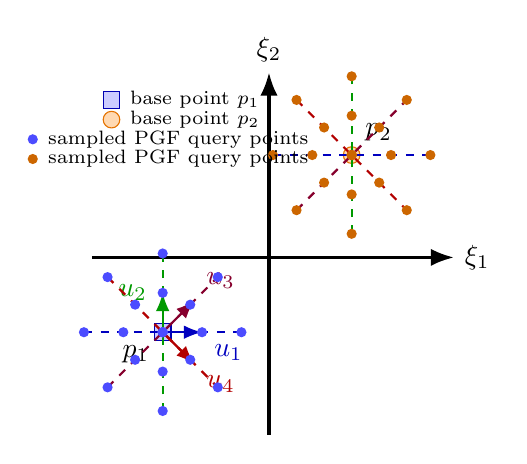
\begin{tikzpicture}[scale=0.50, >=Latex]

\usetikzlibrary{calc,arrows.meta,shapes.misc}

% ----------------------------
% Styles
% ----------------------------
\tikzset{
    axis/.style={->, very thick},
    sampA/.style={circle, fill=blue!70, inner sep=1.3pt},
    sampB/.style={circle, fill=orange!80!black, inner sep=1.3pt},
    baseA/.style={draw=blue!70!black, fill=blue!20, rectangle, minimum size=6pt, inner sep=0pt},
    baseB/.style={draw=orange!90!black, fill=orange!30, circle, minimum size=6pt, inner sep=0pt},
    dir1/.style={blue!75!black, thick},
    dir2/.style={green!60!black, thick},
    dir3/.style={purple!70!black, thick},
    dir4/.style={red!70!black, thick}
}

% ----------------------------
% Axes
% ----------------------------
\draw[axis] (-4.5,0) -- (4.7,0) node[right] {$\xi_1$};
\draw[axis] (0,-4.5) -- (0,4.7) node[above] {$\xi_2$};

% ----------------------------
% Base points
% ----------------------------
\coordinate (P1) at (-2.7,-1.9);
\coordinate (P2) at ( 2.1, 2.6);

\node[baseA] at (P1) {};
\node[below left=2pt] at (P1) {$p_1$};

\node[baseB] at (P2) {};
\node[above right=2pt] at (P2) {$p_2$};


% ----------------------------
% Direction vectors from p1
% u1 = (1,0), u2 = (0,1), u3 = (1,1), u4 = (1,-1)
% 5 points per direction: ell = -2,-1,0,1,2
% ----------------------------

% horizontal through p1
\draw[dir1, dashed] ($(P1)+(-2,0)$) -- ($(P1)+(2,0)$);
\draw[dir1, ->] (P1) -- ($(P1)+(1.0,0)$) node[below right=1pt] {$u_1$};
\foreach \t in {-2,-1,0,1,2}{
    \node[sampA] at ($(P1)+(\t,0)$) {};
}

% vertical through p1
\draw[dir2, dashed] ($(P1)+(0,-2)$) -- ($(P1)+(0,2)$);
\draw[dir2, ->] (P1) -- ($(P1)+(0,1.0)$) node[left=2pt] {$u_2$};
\foreach \t in {-2,-1,0,1,2}{
    \node[sampA] at ($(P1)+(0,\t)$) {};
}

% diagonal + through p1
\draw[dir3, dashed] ($(P1)+(-1.4,-1.4)$) -- ($(P1)+(1.4,1.4)$);
\draw[dir3, ->] (P1) -- ($(P1)+(0.8,0.8)$) node[above right=1pt] {$u_3$};
\foreach \t in {-2,-1,0,1,2}{
    \node[sampA] at ($(P1)+\t*(0.7,0.7)$) {};
}

% diagonal - through p1
\draw[dir4, dashed] ($(P1)+(-1.4,1.4)$) -- ($(P1)+(1.4,-1.4)$);
\draw[dir4, ->] (P1) -- ($(P1)+(0.8,-0.8)$) node[below right=1pt] {$u_4$};
\foreach \t in {-2,-1,0,1,2}{
    \node[sampA] at ($(P1)+\t*(0.7,-0.7)$) {};
}

% ----------------------------
% Same 4 directions through p2
% ----------------------------

% horizontal through p2
\draw[dir1, dashed] ($(P2)+(-2,0)$) -- ($(P2)+(2,0)$);
\foreach \t in {-2,-1,0,1,2}{
    \node[sampB] at ($(P2)+(\t,0)$) {};
}

% vertical through p2
\draw[dir2, dashed] ($(P2)+(0,-2)$) -- ($(P2)+(0,2)$);
\foreach \t in {-2,-1,0,1,2}{
    \node[sampB] at ($(P2)+(0,\t)$) {};
}

% diagonal + through p2
\draw[dir3, dashed] ($(P2)+(-1.4,-1.4)$) -- ($(P2)+(1.4,1.4)$);
\foreach \t in {-2,-1,0,1,2}{
    \node[sampB] at ($(P2)+\t*(0.7,0.7)$) {};
}

% diagonal - through p2
\draw[dir4, dashed] ($(P2)+(-1.4,1.4)$) -- ($(P2)+(1.4,-1.4)$);
\foreach \t in {-2,-1,0,1,2}{
    \node[sampB] at ($(P2)+\t*(0.7,-0.7)$) {};
}

% ----------------------------
% Small legend
% ----------------------------
\node[baseA, label=right:{\scriptsize base point $p_1$}] at (-4.0,4.0) {};
\node[baseB, label=right:{\scriptsize base point $p_2$}] at (-4.0,3.50) {};
\node[sampA, label=right:{\scriptsize sampled PGF query points}] at (-6.0,3.0) {};
\node[sampB, label=right:{\scriptsize sampled PGF query points}] at (-6.0,2.50) {};

\end{tikzpicture}
\caption{Two-dimensional illustration of the random-base line sampling strategy. Two base points $p_1$ and $p_2$ are chosen randomly. Around each base point, four directions are probed, and five query locations are sampled along each direction. For visual clarity, the line samples are drawn symmetrically around the base point; the algorithm only requires consecutive samples along each direction.}
\label{fig:2d_sampling_scheme}
\end{figure}

\section{Experiments}
\label{sec:experiments}

The experiments evaluate whether PGF--JESPRIT provides an accurate and scalable estimator for finite Poisson mixtures. 
We explicitly distinguish algorithmic comparisons from model-level comparisons. 
In the algorithmic setting, all methods target the same finite product-Poisson mixture model in \eqref{eq:model}. 
In the model-level setting, we also report results for alternative count-data models, such as Poisson--Gamma variants, but these are not interpreted as direct algorithmic baselines for PGF--JESPRIT.

\paragraph{Synthetic mixtures.}
We generate $n$ independent samples from the finite Poisson mixture model in \eqref{eq:model}. 
The protocol varies the number of components $K$, the dimension $d$, the sample size $n$, the separation between rate vectors, and the dynamic range of the Poisson rates. 
We consider three representative regimes:
\begin{itemize}[leftmargin=*]
    \item \emph{Separated components}, where the rate vectors are well separated and parameter recovery should be feasible;
    \item \emph{Overlapping components}, where several rate vectors are close and the inverse problem becomes harder;
    \item \emph{Under-specified fitting}, where the fitted number of components is smaller than the true one, to test robustness under model mismatch.
\end{itemize}
\todo{Insert the final experimental grid, e.g., $K\in\{2,3,5,10\}$, $d\in\{1,3,10\}$, and $n\in\{10^3,10^4,10^5\}$.}

\paragraph{Compared methods.}
For algorithmic comparison, the main comparator is EM for the finite product-Poisson mixture model in \eqref{eq:model}. 
This comparison keeps the probabilistic model fixed and contrasts likelihood-based inference with the proposed PGF-sketching and spectral-recovery pipeline. 
We also report runtime and memory usage to assess the benefit of replacing repeated likelihood-based fitting by a fixed-size sketch followed by spectral recovery. 
A coordinate-wise PGF--ESPRIT variant may be included only as an ablation of the proposed spectral pipeline, in order to quantify the effect of the global subspace estimation and joint diagonalization.

When Gamma-regularized or Poisson--Gamma EM variants are included, they are reported separately as model-level comparators. 
These variants can be useful on overdispersed real count data, but they do not isolate the effect of the inference algorithm because they rely on different probabilistic assumptions or regularization criteria.

\paragraph{Metrics.}
On synthetic data, where the ground truth is known, we report the relative error on the rate matrix and on the mixture weights after optimal component matching. 
For both synthetic and real data, we report the PGF reconstruction error, the Hellinger distance between empirical and regenerated marginal distributions, a stabilized chi-square distance, runtime, and peak memory. 
The distributional metrics are computed per coordinate and then averaged over dimensions.

\paragraph{Sketch parameters.}
The PGF--JESPRIT estimator is controlled by the number of sampling directions $M$, the number of PGF samples per direction $L$, and the sampling scale $\Delta$. 
Unless otherwise stated, these parameters are fixed across trials. 
We additionally report a short sensitivity study with respect to $\Delta$, since it controls the trade-off between numerical conditioning and phase wrapping. 
Too small a value of $\Delta$ makes the exponential nodes difficult to separate, while too large a value may introduce phase ambiguities and unstable PGF evaluations.

\begin{table}[t]
\centering
\caption{Synthetic algorithmic comparison under the finite product-Poisson mixture model. Errors are reported as mean $\pm$ standard deviation over independent trials.}
\label{tab:synthetic}
\begin{tabular}{llccc}
\toprule
Regime & Method & Rate err. & Weight err. & PGF err. \\
\midrule
Separated & Poisson EM & \todo{--} & \todo{--} & \todo{--} \\
Separated & PGF--JESPRIT & \todo{--} & \todo{--} & \todo{--} \\
\midrule
Overlap & Poisson EM & \todo{--} & \todo{--} & \todo{--} \\
Overlap & PGF--JESPRIT & \todo{--} & \todo{--} & \todo{--} \\
\midrule
Underfit & Poisson EM & \todo{--} & \todo{--} & \todo{--} \\
Underfit & PGF--JESPRIT & \todo{--} & \todo{--} & \todo{--} \\
\bottomrule
\end{tabular}
\end{table}

\begin{figure}[t]
    \centering
    \includegraphics[width=\linewidth]{figures/runtime_vs_n.pdf}
    \caption{Runtime as a function of the number of samples $n$ for fixed $K$ and $d$. 
    PGF--JESPRIT separates the data-dependent sketching step from the fixed-size spectral recovery step.}
    \label{fig:runtime}
\end{figure}

\paragraph{Real count data.}
We include small real-data checks on the Affairs count dataset \cite{fair1978affairs} and selected high-count genes from the PBMC3k single-cell RNA-seq benchmark \cite{pbmc3k}. 
These experiments are not intended to claim that finite Poisson mixtures are universally valid generative models for these datasets. 
Rather, they test whether the fitted mixtures reproduce realistic count histograms, including sparsity, imbalance, and overdispersion. 
On these datasets, Poisson--Gamma variants may be reported as model-level comparators, separately from the finite-Poisson algorithmic comparison.

\begin{table}[t]
\centering
\caption{Goodness-of-fit on real count datasets. Poisson--Gamma variants, when included, are model-level comparators rather than direct algorithmic baselines.}
\label{tab:real}
\begin{tabular}{llccc}
\toprule
Dataset & Method & $K$ & Hellinger & PGF err. \\
\midrule
Affairs & Finite Poisson EM & \todo{--} & \todo{--} & \todo{--} \\
Affairs & PGF--JESPRIT & \todo{--} & \todo{--} & \todo{--} \\
Affairs & Poisson--Gamma EM & \todo{optional} & \todo{optional} & \todo{optional} \\
\midrule
PBMC3k & Finite Poisson EM & \todo{--} & \todo{--} & \todo{--} \\
PBMC3k & PGF--JESPRIT & \todo{--} & \todo{--} & \todo{--} \\
PBMC3k & Poisson--Gamma EM & \todo{optional} & \todo{optional} & \todo{optional} \\
\bottomrule
\end{tabular}
\end{table}

\paragraph{Discussion.}
\todo{Replace this paragraph by the final numerical findings.}
We expect PGF--JESPRIT to be most effective in regimes where the mixture has a moderate number of components and the rate vectors are sufficiently separated. 
In such settings, the empirical PGF has a clear exponential structure and the joint subspace estimation should recover coherent multidimensional components. 
The main computational advantage is expected when $n$ is large: once the empirical PGF sketch has been computed, the spectral recovery step depends primarily on the sketch size rather than on the number of observations.

The main limitations are also evaluated experimentally. 
First, the choice of $\Delta$ is critical because it affects both conditioning and phase wrapping. 
Second, large Poisson rates can make PGF evaluations numerically unstable unless the sampling points are chosen carefully. 
Third, unlike EM, the algebraic recovery step does not directly optimize the likelihood; it may therefore obtain a good PGF fit while being less competitive under histogram-based metrics in highly overlapping regimes. 
Finally, comparisons with Poisson--Gamma variants should be interpreted as model-level comparisons, since differences may reflect both the inference procedure and the probabilistic assumptions.

\section{Conclusion}

We presented a scalable framework for scalable mixed Poisson inference from empirical PGF sketches using joint ESPRIT. 
The method compresses count data into transform evaluations, recovers multidimensional rate vectors through a global subspace and joint diagonalization, and estimates mixture weights by constrained least squares. 
The final paper will complete the empirical study by separating algorithmic comparisons under the finite product-Poisson mixture model from model-level comparisons involving alternative count-data models. 
\todo{Add final conclusion once experiments are complete.}

\section*{GenAI Usage Disclosure}
\todo{For the final CIKM submission, replace this placeholder with the exact disclosure required by the ACM/CIKM policy. Example: ``The authors used generative AI tools for language editing and LaTeX drafting assistance. All scientific claims, experiments, code, and final text were verified by the authors.''}

\bibliographystyle{ACM-Reference-Format}
\bibliography{references}

\end{document}